\pdfminorversion=4
\documentclass[aspectratio=169]{beamer}

\mode<presentation>
{
  \usetheme{default}
  \usecolortheme{default}
  \usefonttheme{default}
  \setbeamertemplate{navigation symbols}{}
  \setbeamertemplate{caption}[numbered]
  \setbeamertemplate{footline}[frame number]  % or "page number"
  \setbeamercolor{frametitle}{fg=white}
  \setbeamercolor{footline}{fg=black}
} 

\usepackage[english]{babel}
\usepackage[utf8]{inputenc}
\usepackage{tikz}
\usepackage{courier}
\usepackage{array}
\usepackage{bold-extra}
\usepackage{minted}
\usepackage[thicklines]{cancel}
\usepackage{fancyvrb}

\xdefinecolor{dianablue}{rgb}{0.18,0.24,0.31}
\xdefinecolor{darkblue}{rgb}{0.1,0.1,0.7}
\xdefinecolor{darkgreen}{rgb}{0,0.5,0}
\xdefinecolor{darkgrey}{rgb}{0.35,0.35,0.35}
\xdefinecolor{darkorange}{rgb}{0.8,0.5,0}
\xdefinecolor{darkred}{rgb}{0.7,0,0}
\definecolor{darkgreen}{rgb}{0,0.6,0}
\definecolor{mauve}{rgb}{0.58,0,0.82}

\title[2022-09-08-chess-scientific-python-ecosystem]{Adoption of Python and modern software practices \\ in high energy physics}
\author{Jim Pivarski}
\institute{Princeton University -- IRIS-HEP}
\date{September 8, 2022}

\usetikzlibrary{shapes.callouts}

\begin{document}

\logo{\pgfputat{\pgfxy(0.11, 7.4)}{\pgfbox[right,base]{\tikz{\filldraw[fill=dianablue, draw=none] (0 cm, 0 cm) rectangle (50 cm, 1 cm);}\mbox{\hspace{-8 cm}
\includegraphics[height=1 cm]{princeton-logo-long.png}\hspace{0.1 cm}\raisebox{0.1 cm}{
\includegraphics[height=0.8 cm]{iris-hep-logo-long.png}}\hspace{0.1 cm}}}}}

\begin{frame}
  \titlepage
\end{frame}

\logo{\pgfputat{\pgfxy(0.11, 7.4)}{\pgfbox[right,base]{\tikz{\filldraw[fill=dianablue, draw=none] (0 cm, 0 cm) rectangle (50 cm, 1 cm);}\mbox{\hspace{-8 cm}
\includegraphics[height=1 cm]{princeton-logo.png}\hspace{0.1 cm}\raisebox{0.1 cm}{
\includegraphics[height=0.8 cm]{iris-hep-logo.png}}\hspace{0.1 cm}}}}}

% Uncomment these lines for an automatically generated outline.
%\begin{frame}{Outline}
%  \tableofcontents
%\end{frame}

% START START START START START START START START START START START START START

\begin{frame}{Subject of this talk: a rough assortment of things}
\vspace{0.5 cm}

\begin{itemize}\setlength{\itemsep}{0.5 cm}
\item Adoption of Python in high energy physics (HEP)

\vspace{0.1 cm}
\begin{itemize}\setlength{\itemsep}{0.25 cm}
\item How Python is used in HEP, trend toward Python for data analysis
\end{itemize}

\item Adoption of ``modern software practices'' (devops)

\vspace{0.1 cm}
\begin{itemize}\setlength{\itemsep}{0.25 cm}
\item Source control: git/GitHub/GitLab
\item Automated tests: continuous integration (CI), continuous deployment (CD)
\item Modularity of packages: Lego-style analysis
\item Package management: pip, conda
\item Environment encapsulation: venv, conda, Docker
\item Social structures: silos versus mixing
\end{itemize}

\end{itemize}
\end{frame}

\begin{frame}{Is Python part of that ``modern''?}
\large
\vspace{0.25 cm}
Python is leading every programming language popularity index.
\vspace{0.25 cm}
\begin{columns}[t]
\column{0.33\linewidth}
\centering Tiobe
\vspace{0.1 cm}
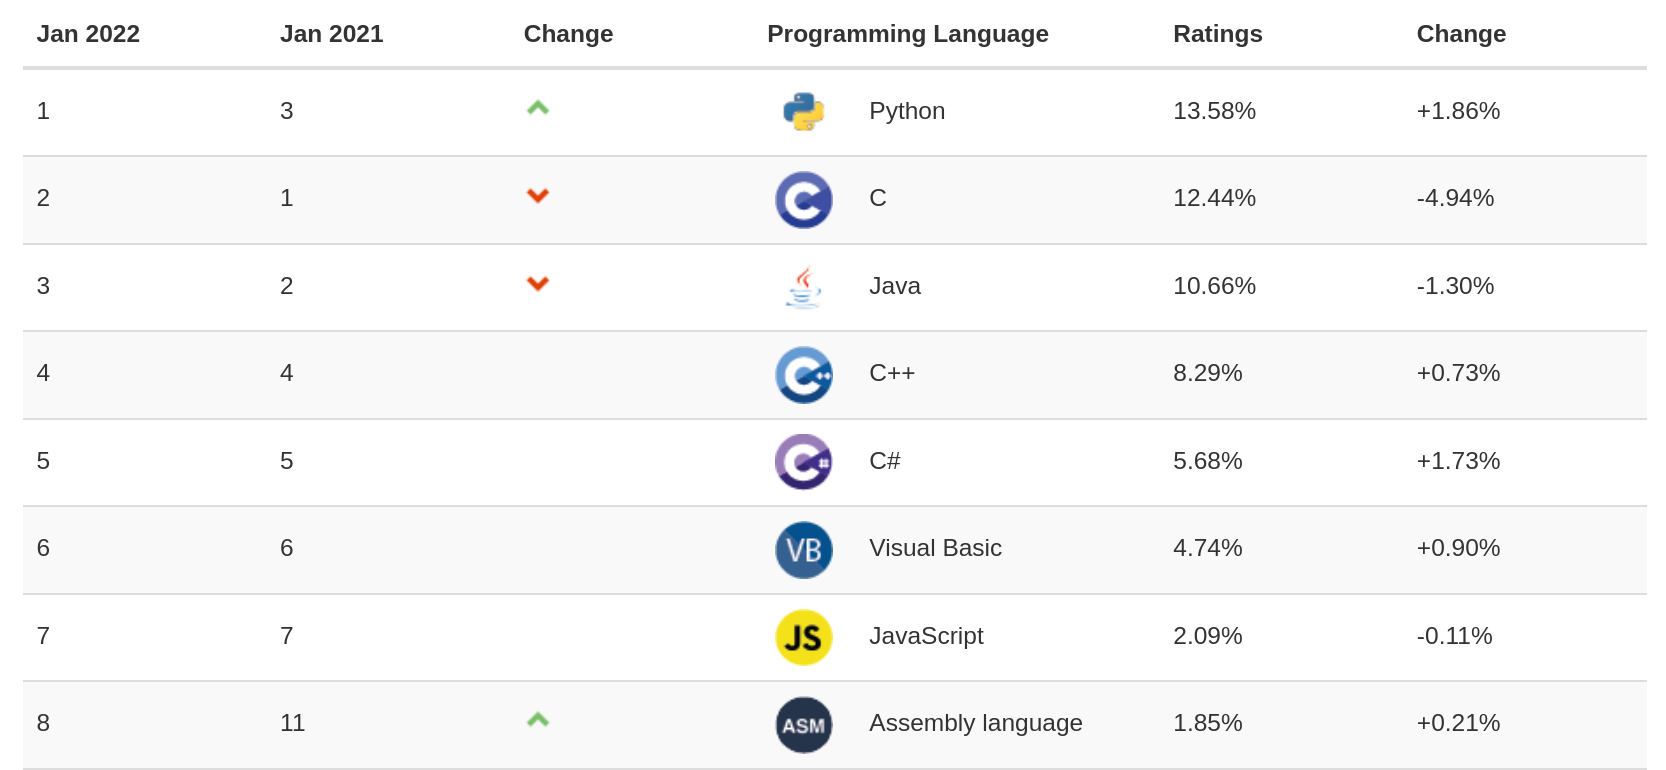
\includegraphics[width=\linewidth]{PLOTS/python-rankings-tiobe-2022.png}
\column{0.33\linewidth}
\centering PYPL
\vspace{0.1 cm}
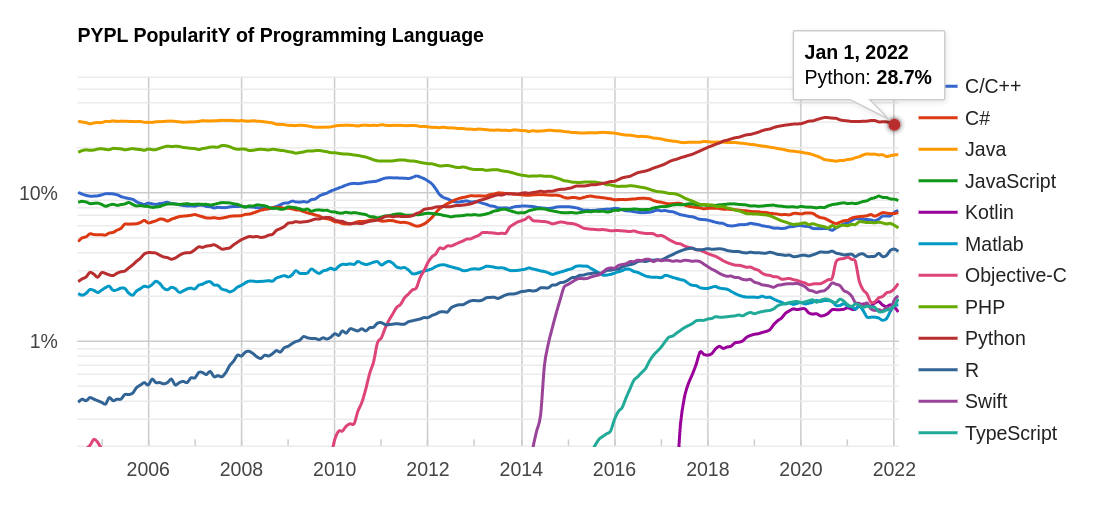
\includegraphics[width=\linewidth]{PLOTS/python-rankings-pypl-2022.png}
\column{0.33\linewidth}
\centering Google Trends
\vspace{0.1 cm}
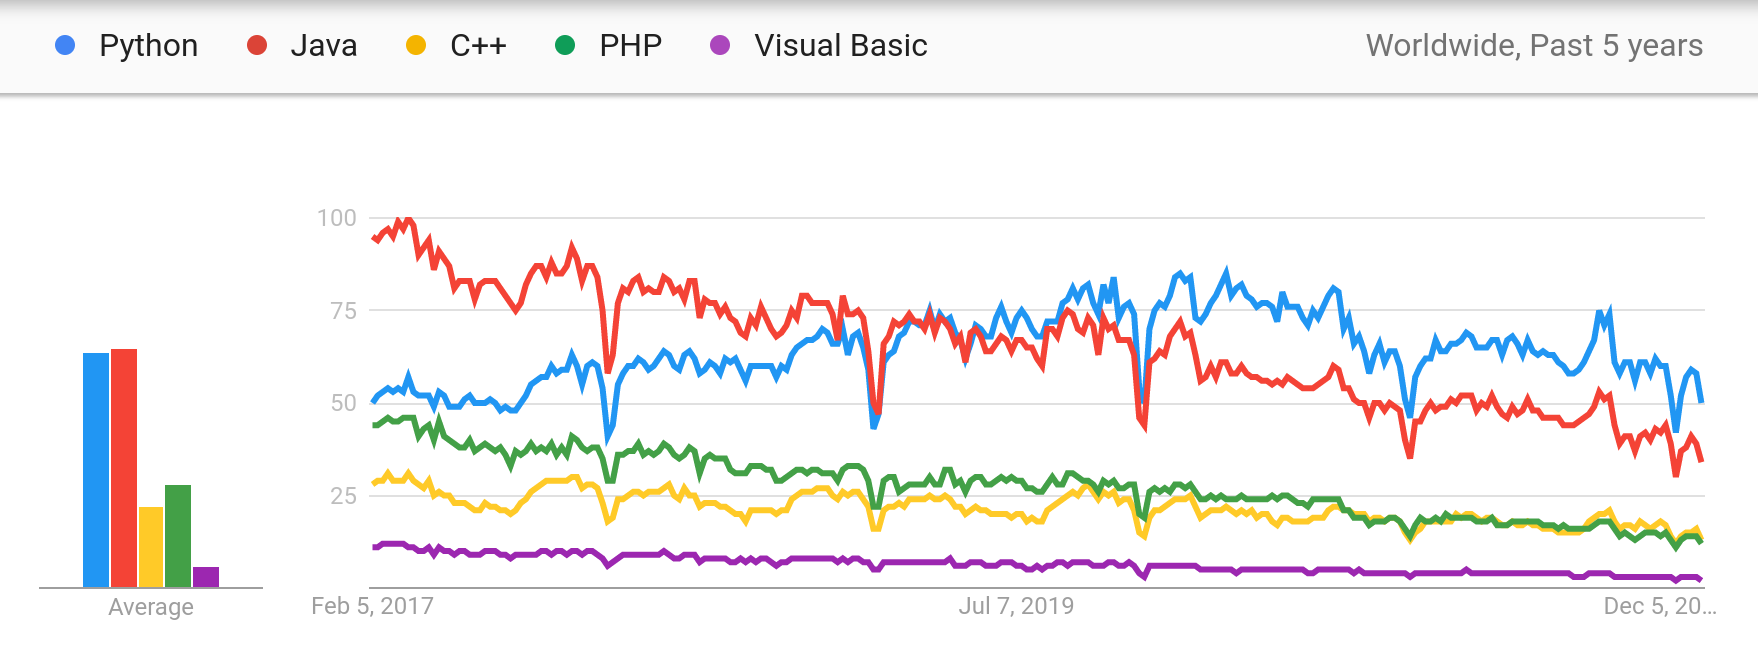
\includegraphics[width=\linewidth]{PLOTS/python-rankings-googletrends-2022.png}
\end{columns}
\vspace{0.25 cm}
\begin{columns}[t]
\column{0.5\linewidth}
\centering GitHut
\vspace{0.1 cm}
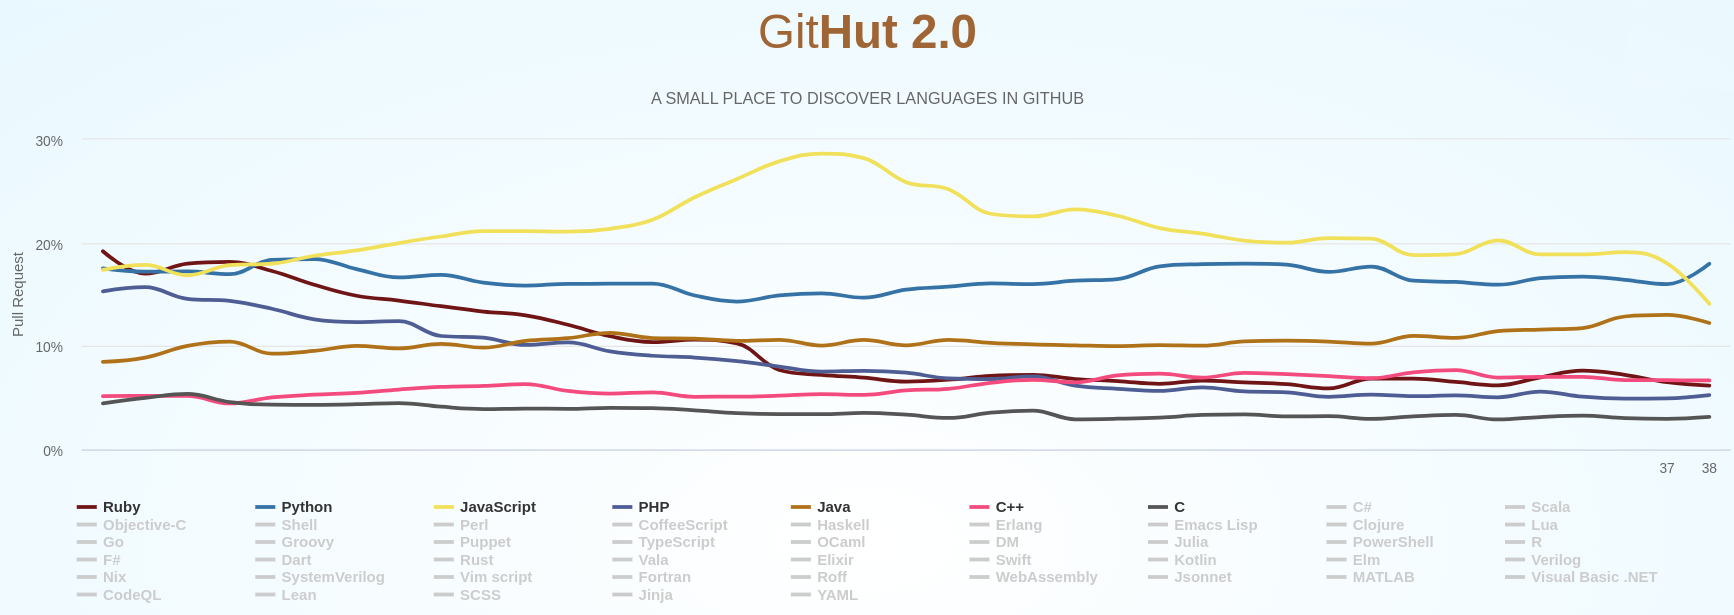
\includegraphics[width=\linewidth]{PLOTS/python-rankings-githut-2022.png}
\column{0.45\linewidth}
\centering StackOverflow
\vspace{0.1 cm}
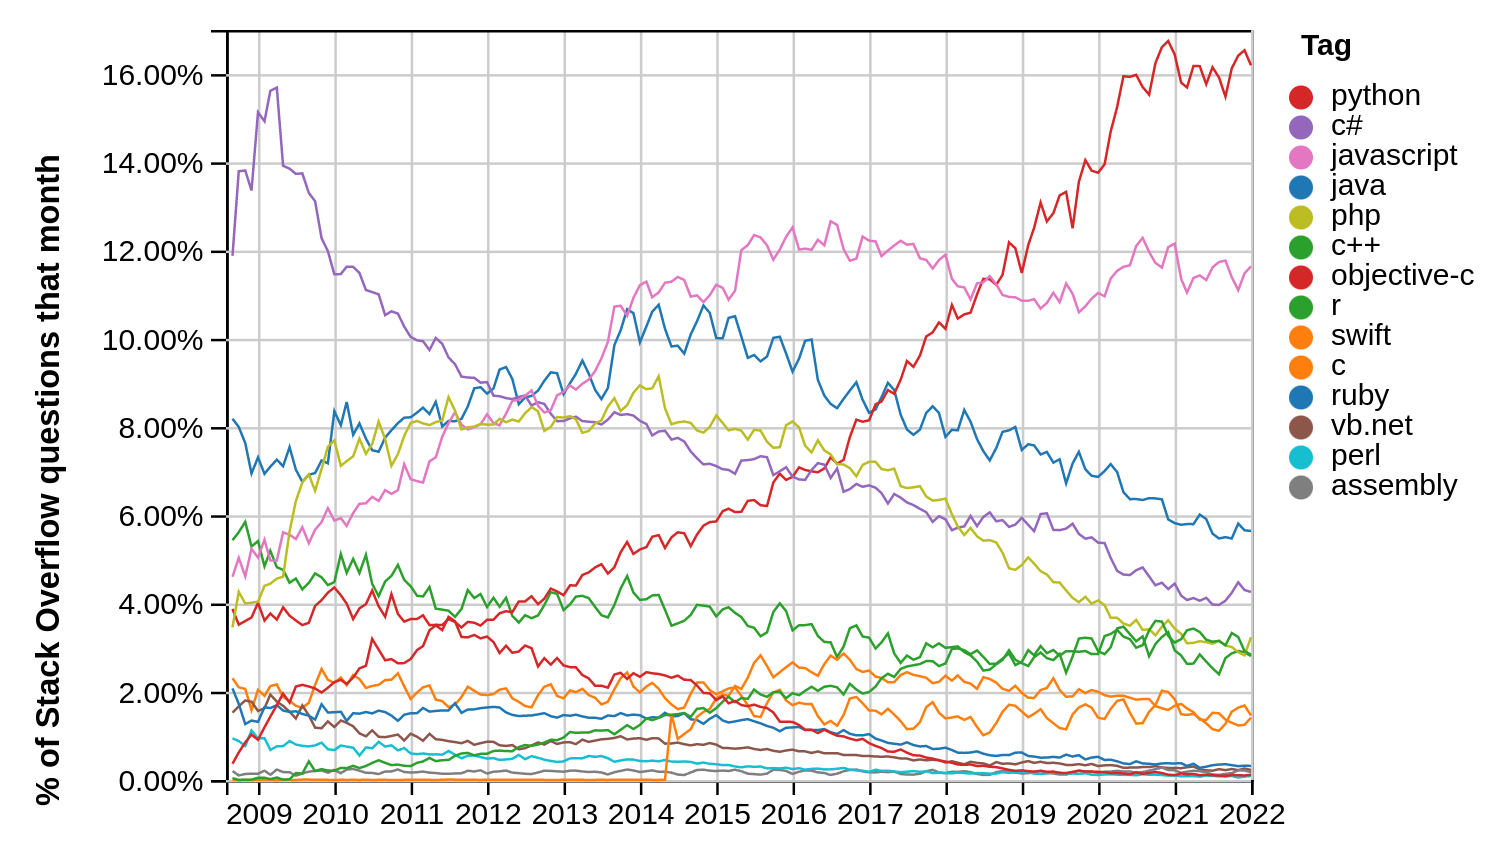
\includegraphics[width=\linewidth]{PLOTS/python-rankings-stackoverflow-2022.png}
\end{columns}
\end{frame}

\begin{frame}{Is Python part of that ``modern''?}
\large
\vspace{0.25 cm}

And this is a recent thing, too.

\vspace{0.25 cm}
\href{https://www.tiobe.com/tiobe-index/}{\textcolor{blue}{Tiobe index}}'s top 3 or 4 for the past 35 years:

\renewcommand{\arraystretch}{1.25}
\begin{center}
\begin{tabular}{c l l}
1987 & C, Lisp, Prolog                 & \\
1992 & C, C++, Pascal                  & Python exists \\
1997 & C, C++, (Visual) Basic          & Python is \#28 \\
2002 & Java, C, C++, (Visual) Basic    & Python is \#12 \\
2007 & Java, C, C++, (Visual) Basic    & Python is \#7 \\
2012 & Java, C, C++, C\#               & Python is \#8 \\
2017 & Java, C, C++, C\#               & Python is \#5 \\
2022 & Python, C, Java, C++            & Python is \#1 \\
\end{tabular}
\end{center}
\end{frame}

\begin{frame}{Not all programmers are data analysts: what about us?}
\vspace{0.25 cm}

Google search trends for language name + ``analytics'' or ``machine learning.''

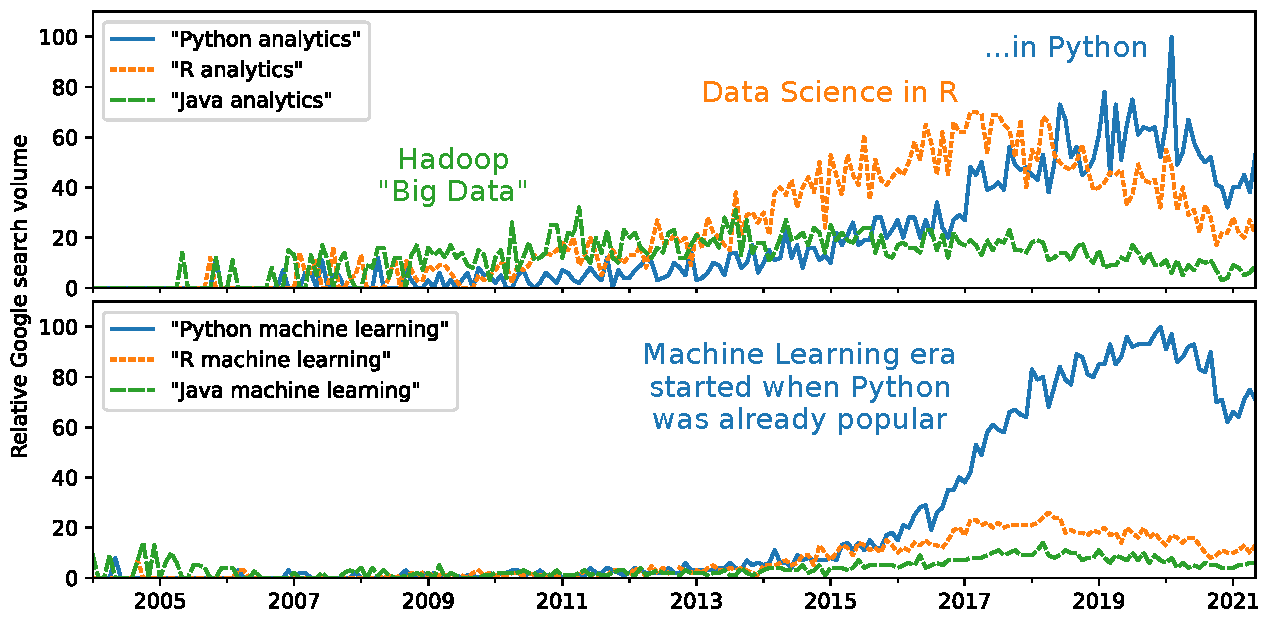
\includegraphics[width=\linewidth]{PLOTS/analytics-by-language.pdf}
\end{frame}

\begin{frame}{Not all data analysts are physicists: what about us?}
\vspace{0.25 cm}

Regex matches to all Computing in High Energy Physics (CHEP) titles and abstracts.

\vspace{-0.1 cm}
\begin{center}
\only<1>{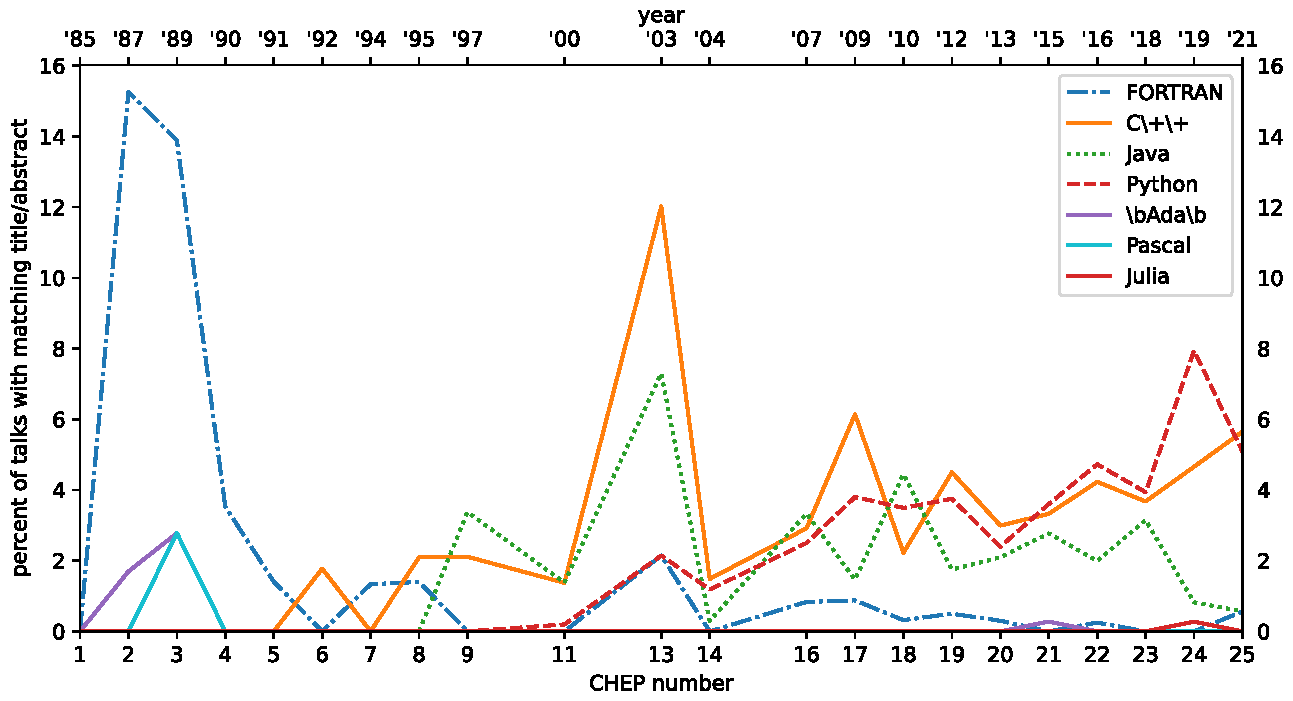
\includegraphics[width=0.95\linewidth]{PLOTS/chep-papers-language.pdf}}\only<2>{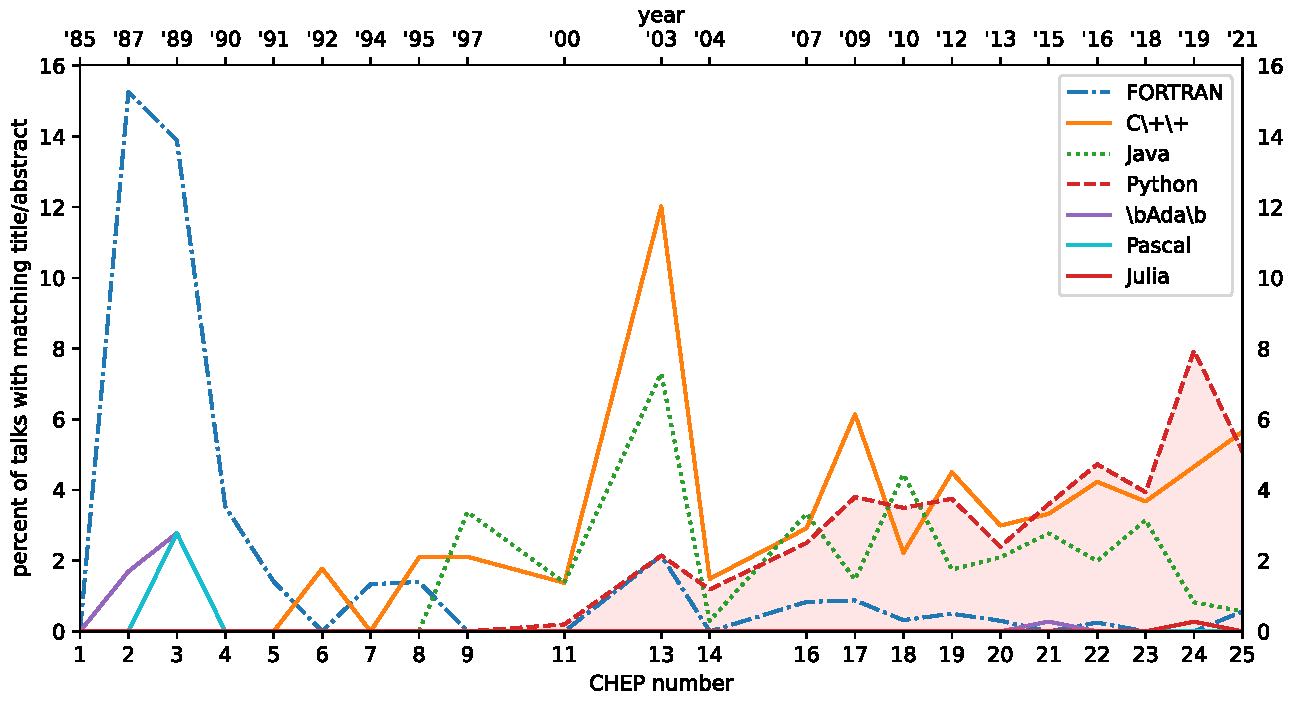
\includegraphics[width=0.95\linewidth]{PLOTS/chep-papers-language-shaded.pdf}}
\end{center}
\end{frame}

\begin{frame}{Lucas Taylor, summary of data analysis track, CHEP 2001}
\vspace{0.25 cm}

\mbox{ } \hfill 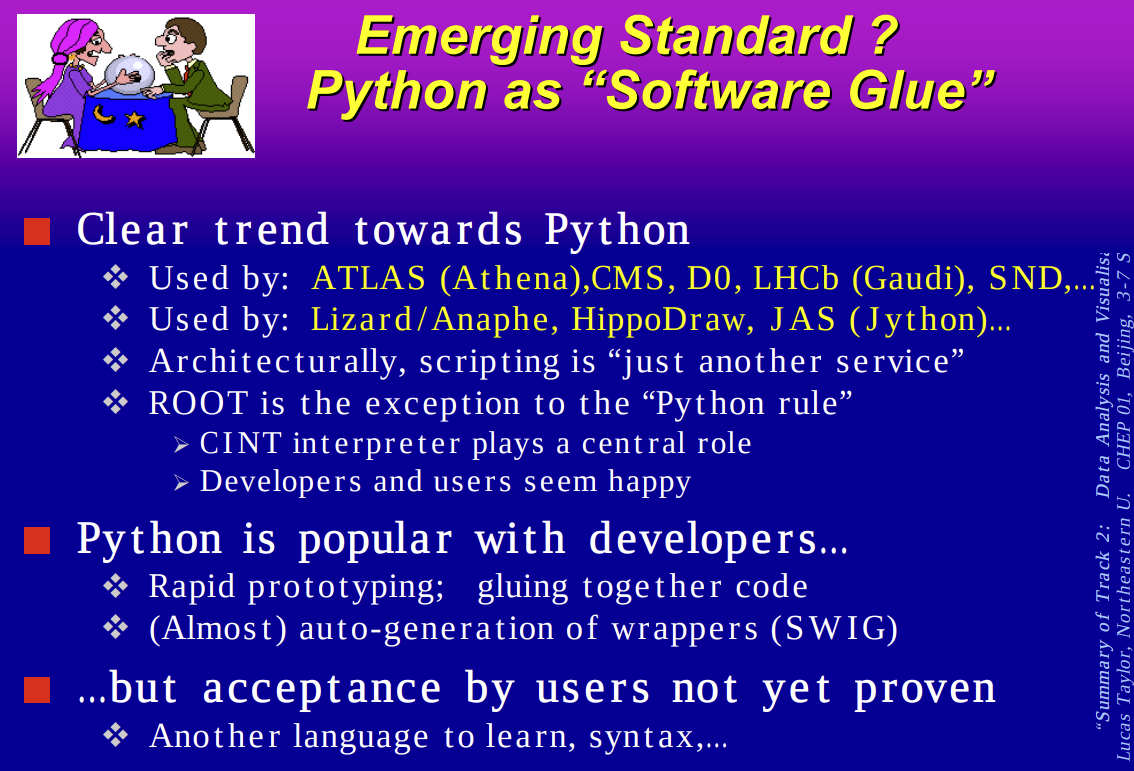
\includegraphics[width=0.82\linewidth]{PLOTS/chep-2001-python.png} \hfill \mbox{ }
\end{frame}

\begin{frame}{}
\vspace{1 cm}
\Large

\begin{center}
But note the emphasis on ``glue'' and ``configuration,''

\vspace{0.1 cm}
not the process of analyzing data.

\vspace{1 cm}
How do physicists {\it use} Python?
\end{center}
\end{frame}

\begin{frame}{Analysis of 11\,635 GitHub repos created by 2\,172 physicists}
\vspace{0.25 cm}

Software for the CMS experiment is on GitHub and all CMS physicists need to fork it. Using that, we can identify all of those physicists' non-fork, public repositories.

\vspace{0.2 cm}

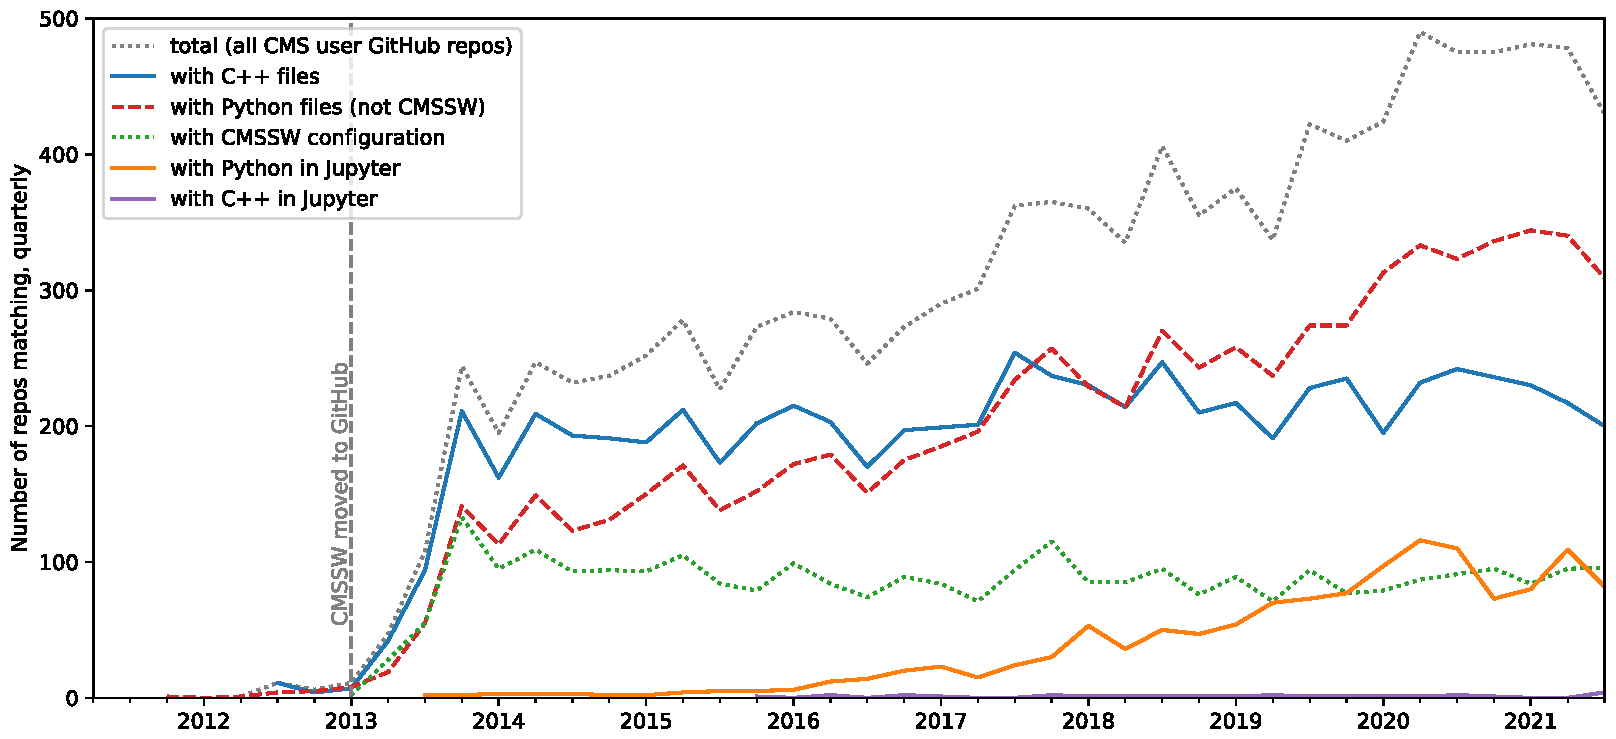
\includegraphics[width=\linewidth]{PLOTS/gihub-language-fullstudy.pdf}
\end{frame}

\begin{frame}{Analysis of 11\,635 GitHub repos created by 2\,172 physicists}
\vspace{0.25 cm}

By regex searching for ``\mintinline{python}{import [A-Za-z_][A-Za-z_0-9]*}'' etc., we can count the number of physicist repositories that use different packages over time.

\vspace{0.2 cm}

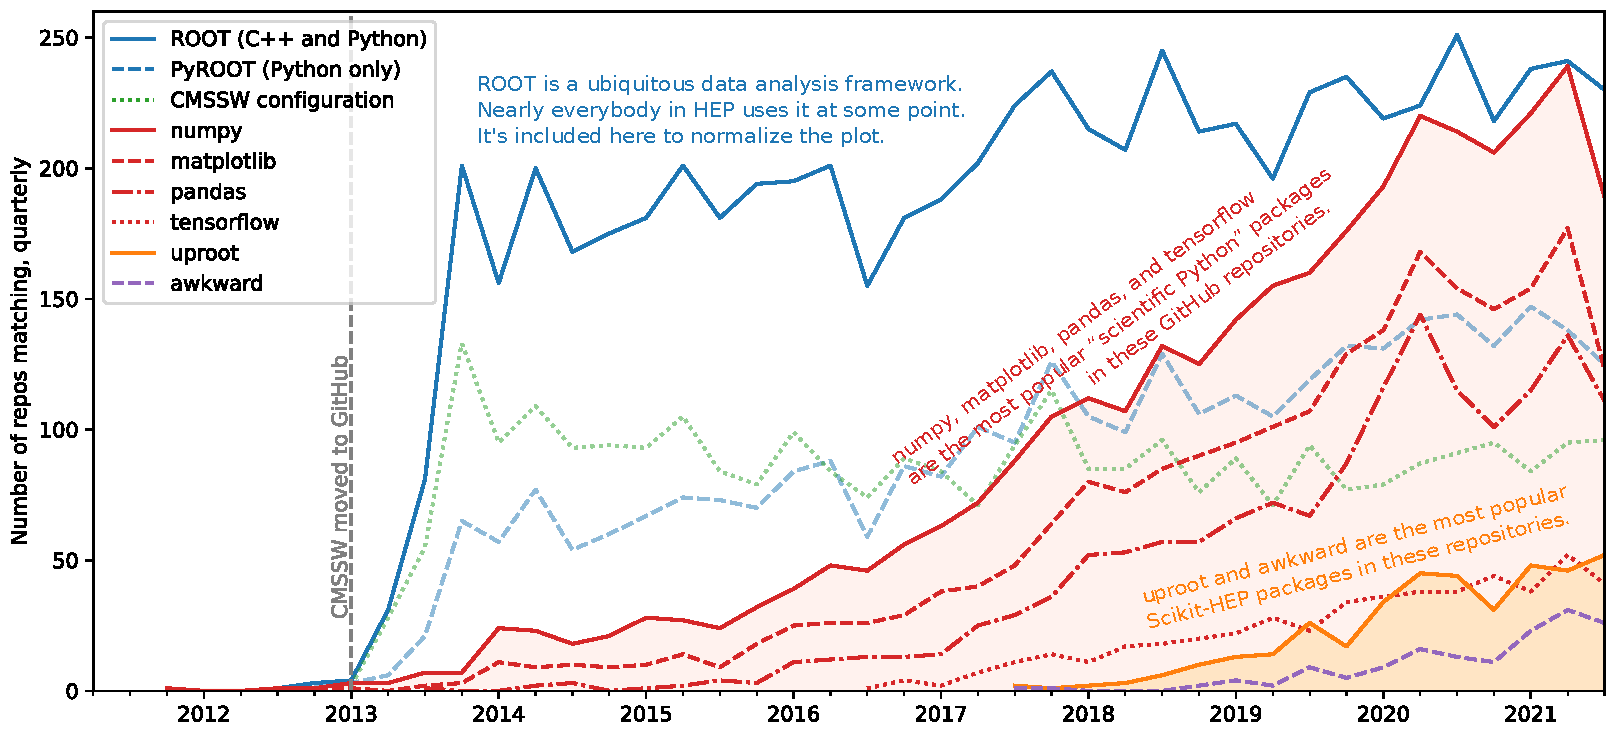
\includegraphics[width=\linewidth]{PLOTS/gihub-package-fullstudy.pdf}
\end{frame}

\begin{frame}{You can also just ask them: PyHEP 2020 survey ($N=406$)}
\vspace{0.5 cm}
\begin{columns}
\column{1.15\linewidth}
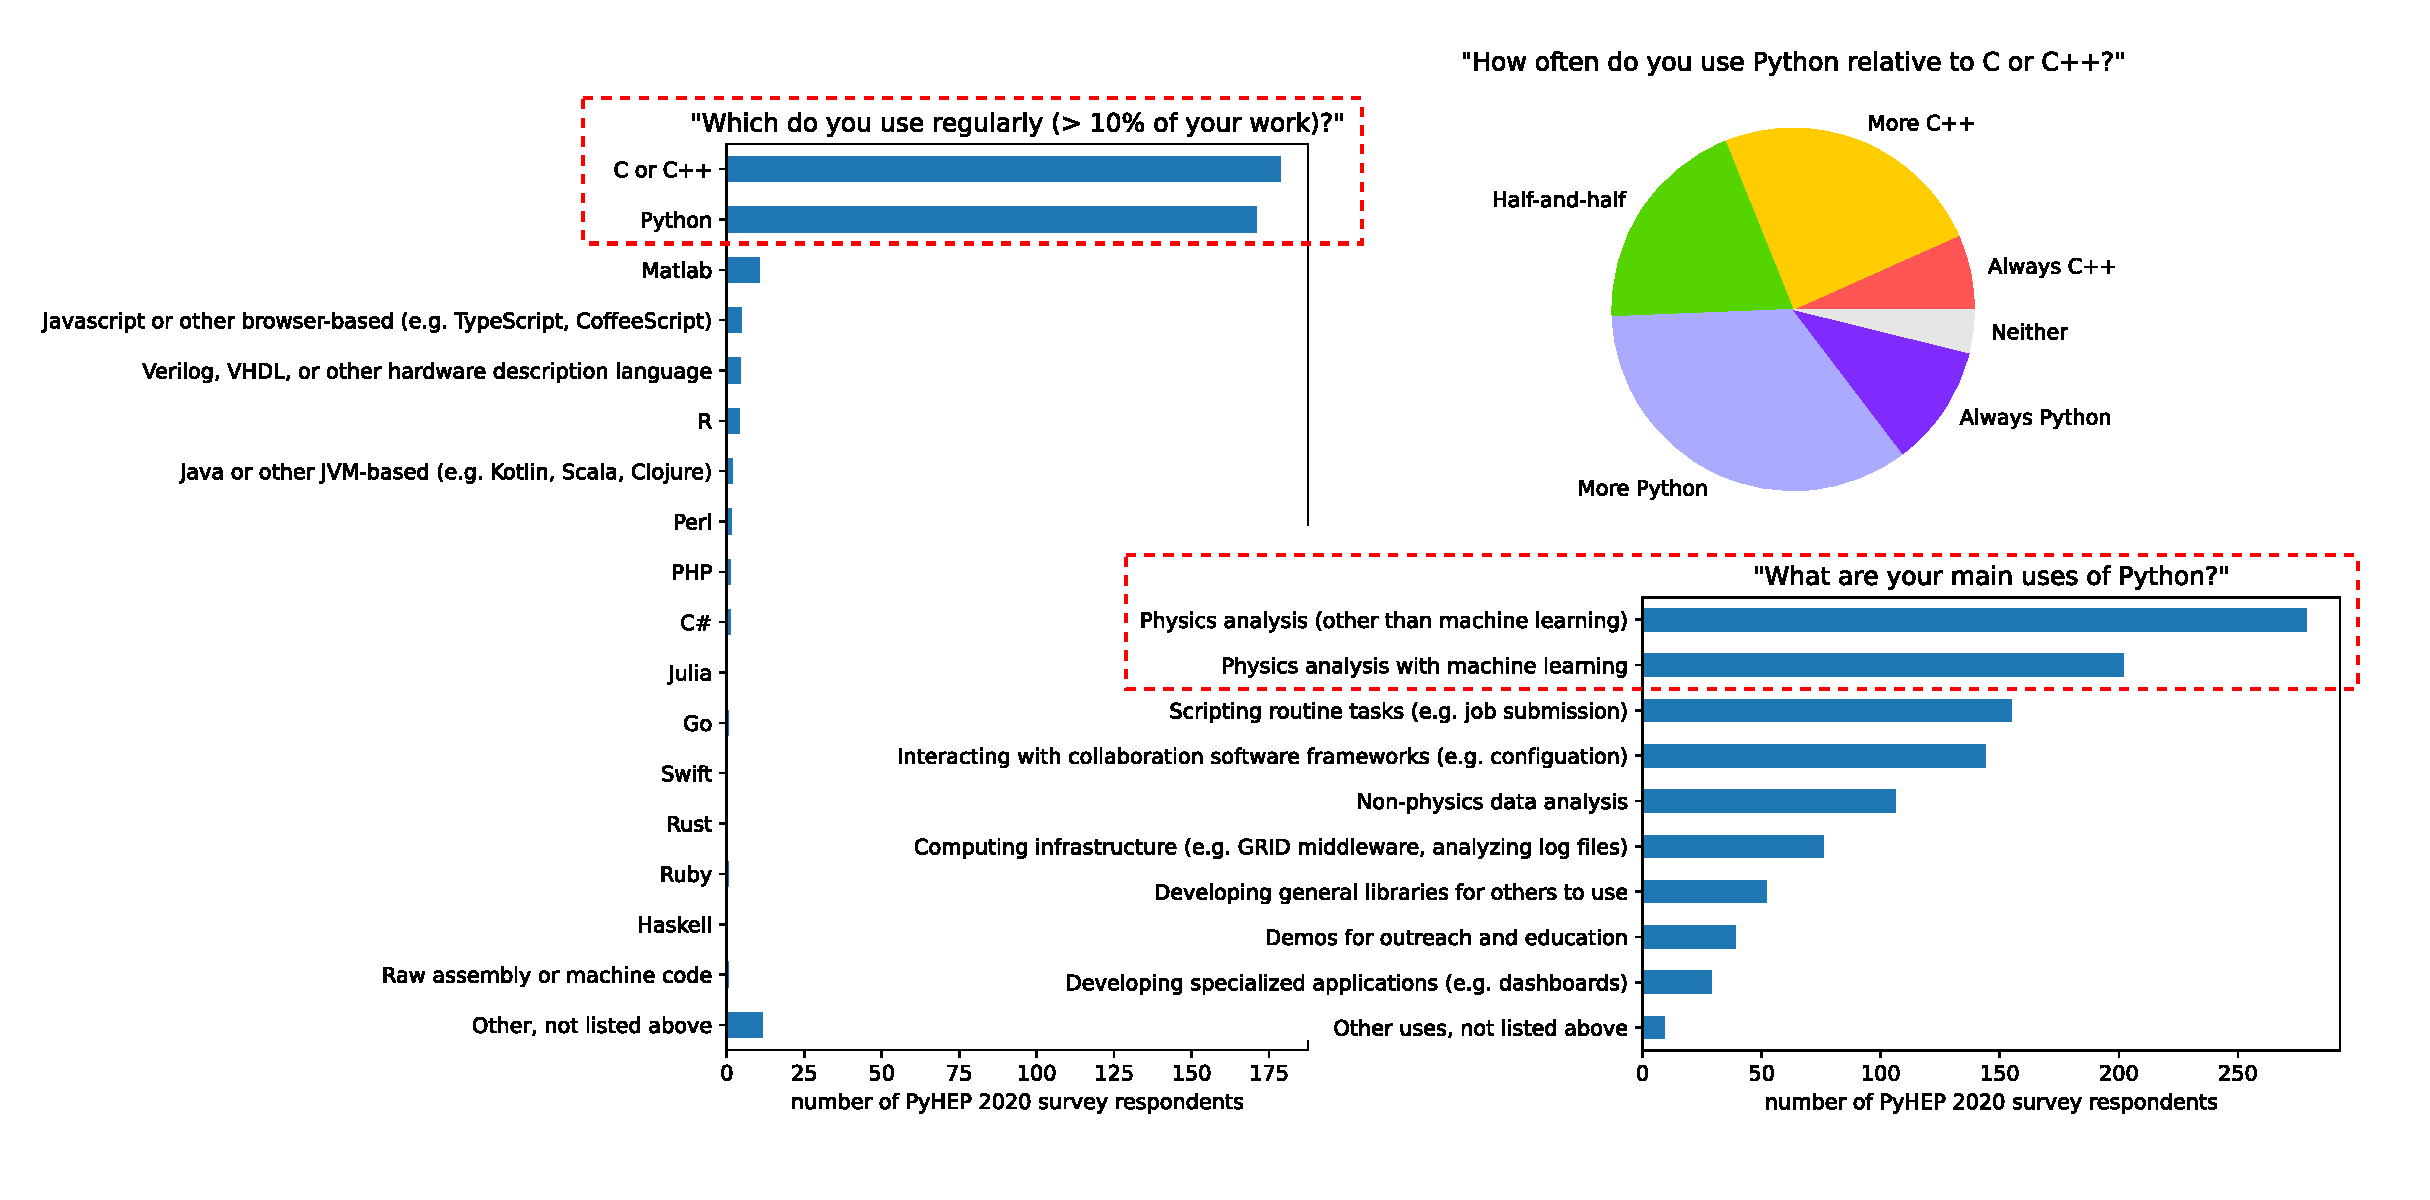
\includegraphics[width=\linewidth]{PLOTS/pyhep2020-survey-5.pdf}
\end{columns}
\end{frame}

\begin{frame}{There has been a massive adoption of Python for HEP analysis.}
\large
\vspace{0.35 cm}

{\Large Why does it matter?}

\vspace{0.25 cm}
\uncover<2->{Humans use programming languages to communicate technical issues with each other as much as with computers. Cultures develop around them.}

\vspace{0.25 cm}
\begin{uncoverenv}<3->
\begin{onlyenv}<3-9>
\begin{itemize}\setlength{\itemsep}{0.1 cm}
\item<3-> \textcolor{darkblue}{Python}: culture of readability first, performance and software architecture later, if at all. More focus on the domain (e.g.\ science) than programming.
\item<4-> \textcolor{darkblue}{C++}: performance and software architecture are up-front concerns; favored among large-scale HEP processing, high-speed trading, game engines.
\item<5-> \textcolor{darkblue}{Java} and \textcolor{darkblue}{Go}: software architecture is an overriding concern, especially in networked services; backend web engineers and internal corporate networks.
\item<6-> \textcolor{darkblue}{Rust}: performance with memory safety overrides all.
\item<7-> \textcolor{darkblue}{Julia}: academic/scientist community, but very focused on performance.
\item<8-> \textcolor{darkblue}{Haskell}: theoretical aspects of computing; computer scientists.
\item<9-> \textcolor{darkblue}{C\#}: Windows. \textcolor{darkblue}{Swift}: Mac.
\end{itemize}
\end{onlyenv}\begin{onlyenv}<10>
\mbox{ } \hfill 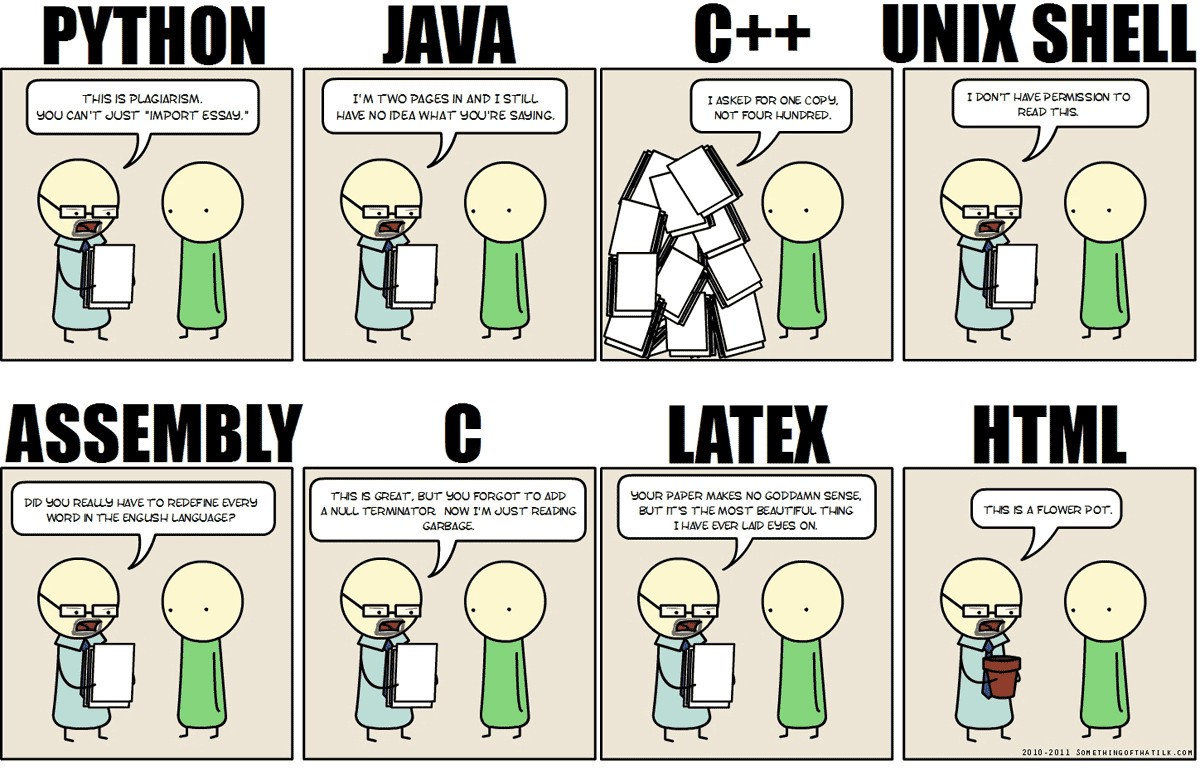
\includegraphics[width=0.63\linewidth]{PLOTS/somethingofthatilk-comic.jpg} \hfill \mbox{ }
\end{onlyenv}
\vspace{8 cm}
\end{uncoverenv}
\end{frame}

\begin{frame}{There has been a massive adoption of Python for HEP analysis.}
\large
\vspace{0.35 cm}

{\Large Why does it matter?}

\vspace{0.5 cm}
We are in closer communication with developers of Python open source projects like NumPy, Scikit-Learn, and AstroPy.

\vspace{0.5 cm}
Large-scale HEP processing frameworks are no longer the default model for how to develop a data analysis package.
\end{frame}

\begin{frame}{Model: small, specialized packages for Lego-style data analysis}
\vspace{0.75 cm}
\Large

\begin{columns}
\column{0.55\linewidth}
\begin{uncoverenv}<1->
\mbox{ } \hfill Scientific Python ecosystem \hfill \mbox{ }

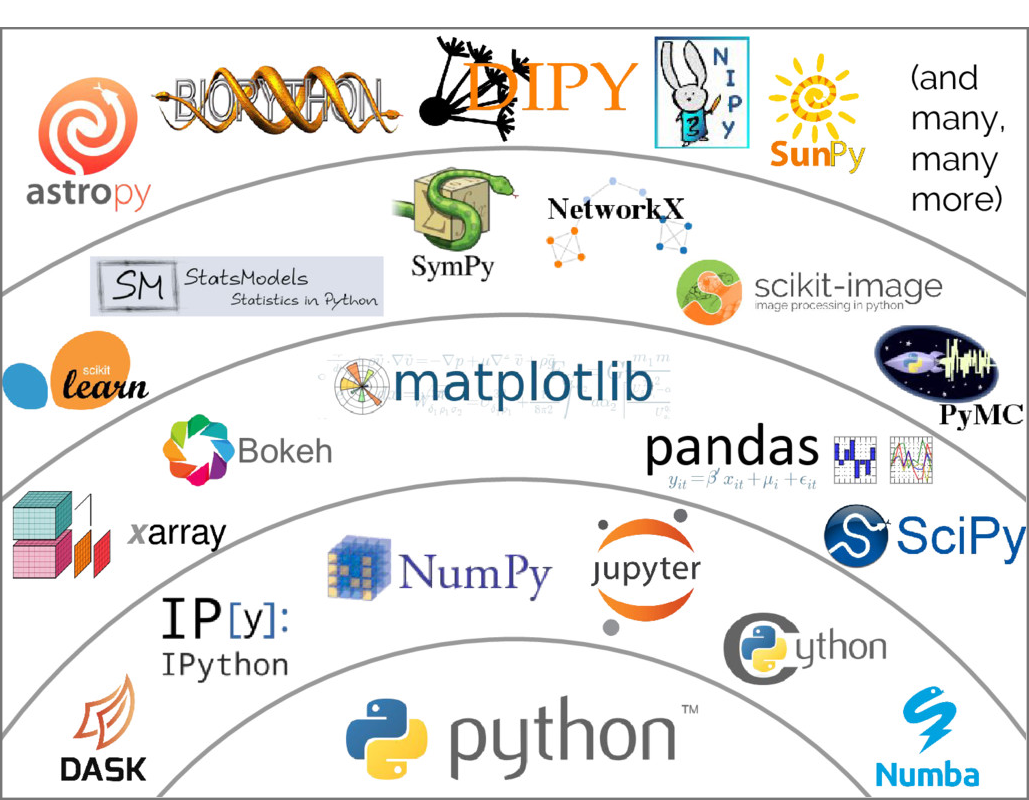
\includegraphics[width=\linewidth]{PLOTS/shells-border.png}
\end{uncoverenv}

\column{0.55\linewidth}
\begin{uncoverenv}<2->
\mbox{ } \hfill Scikit-HEP ecosystem \hfill \mbox{ }

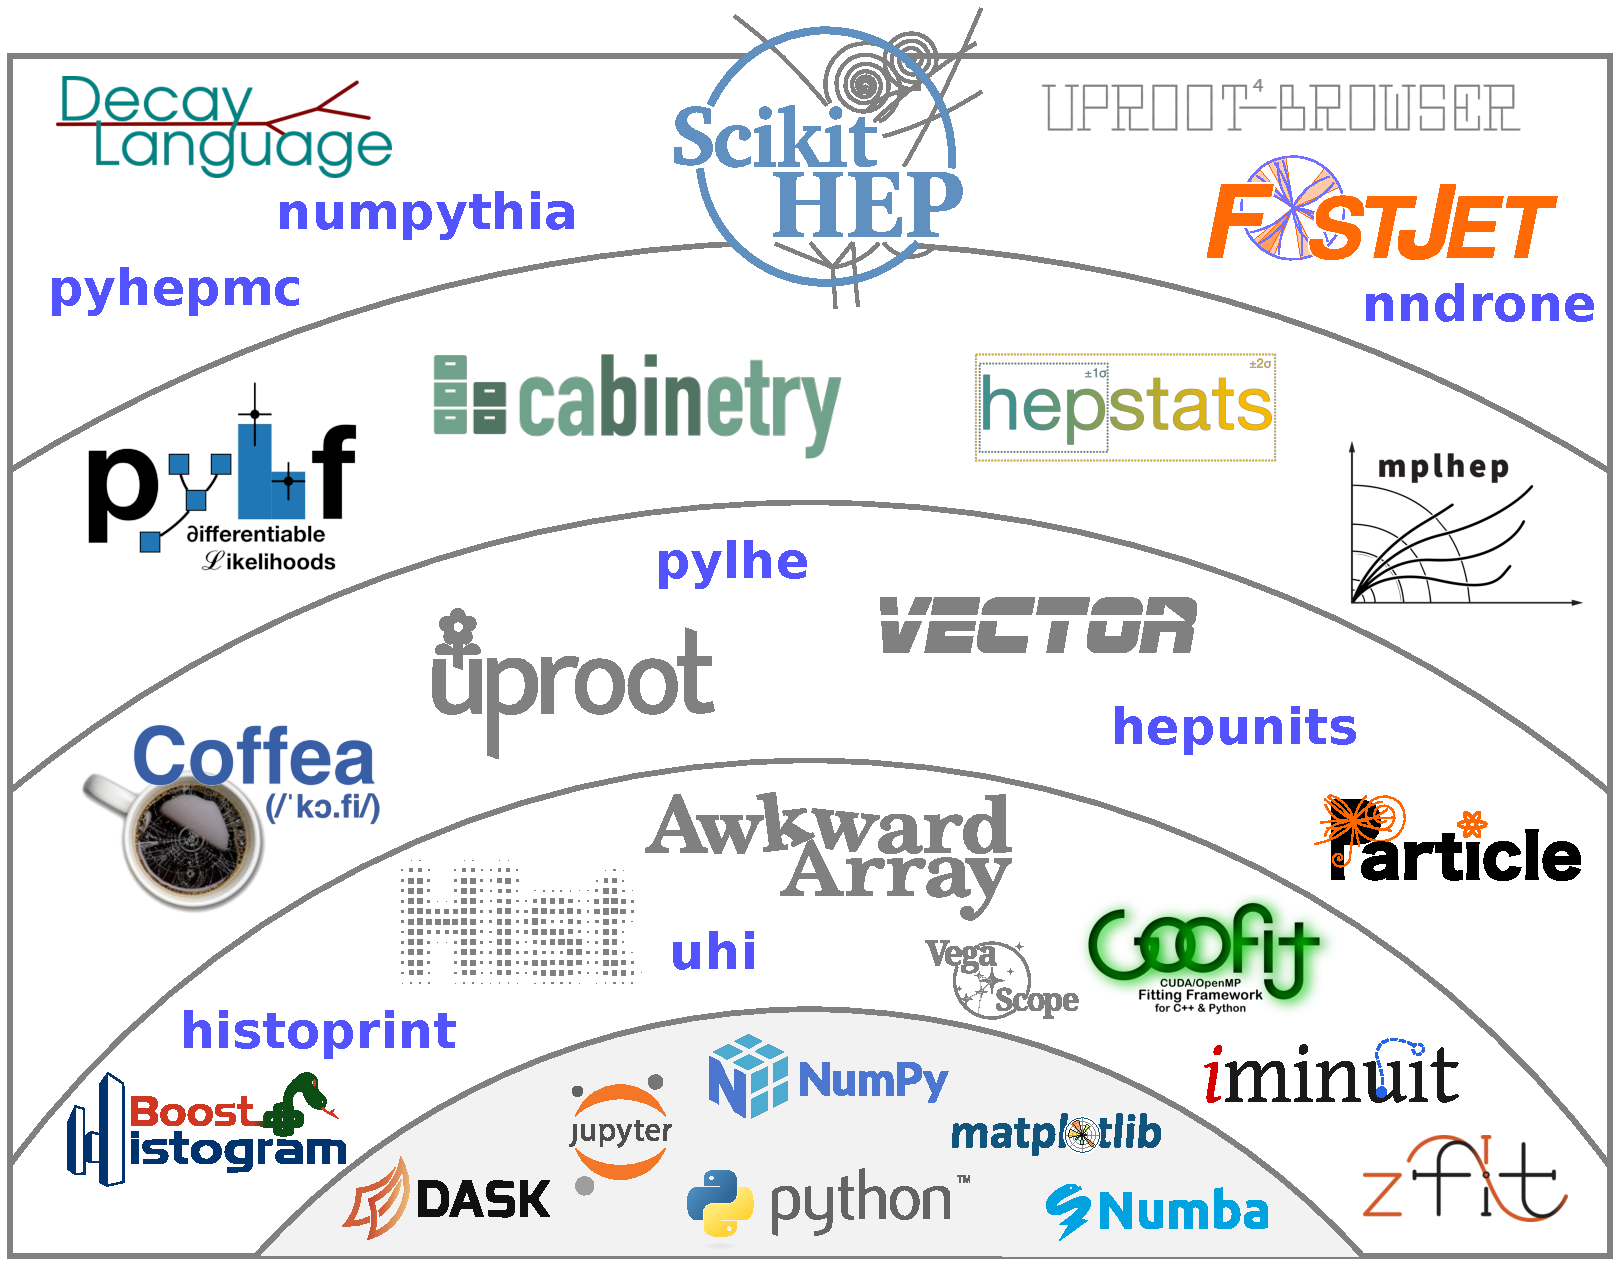
\includegraphics[width=\linewidth]{PLOTS/shells-hep.pdf}
\end{uncoverenv}
\end{columns}
\end{frame}

\begin{frame}{Download rates of Scikit-HEP packages (on Mac \& Windows)}
\vspace{0.25 cm}
\only<1>{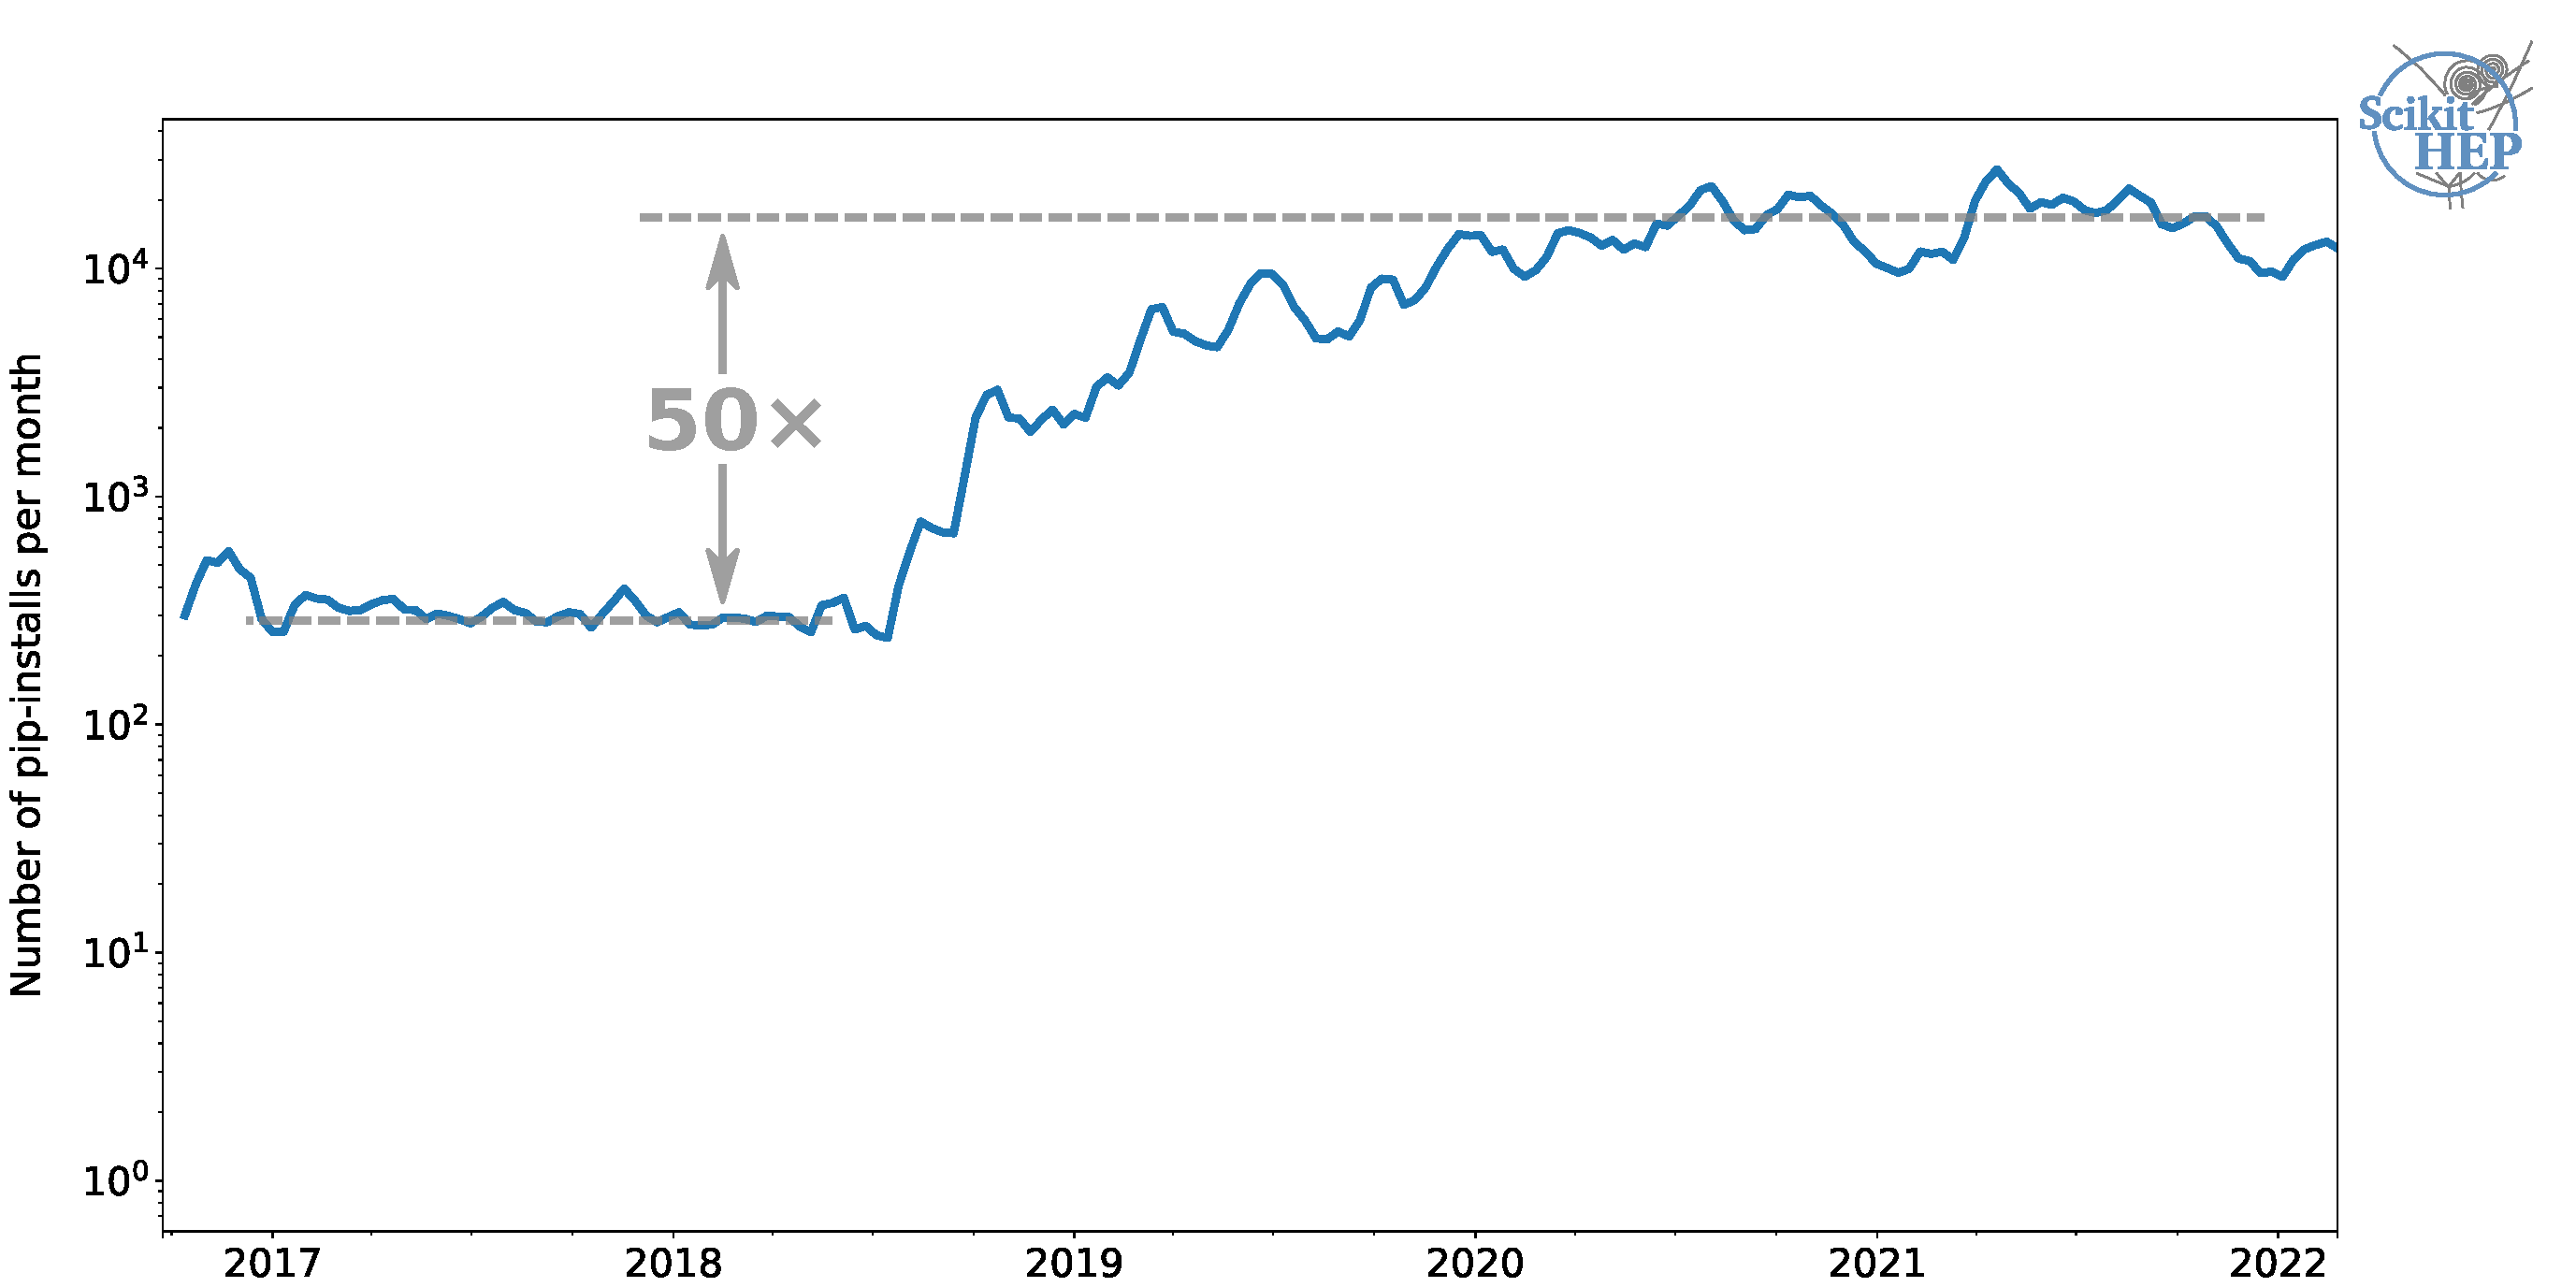
\includegraphics[width=\linewidth]{PLOTS/pip-macwin-scikithep-log-for-report-0.pdf}}\only<2>{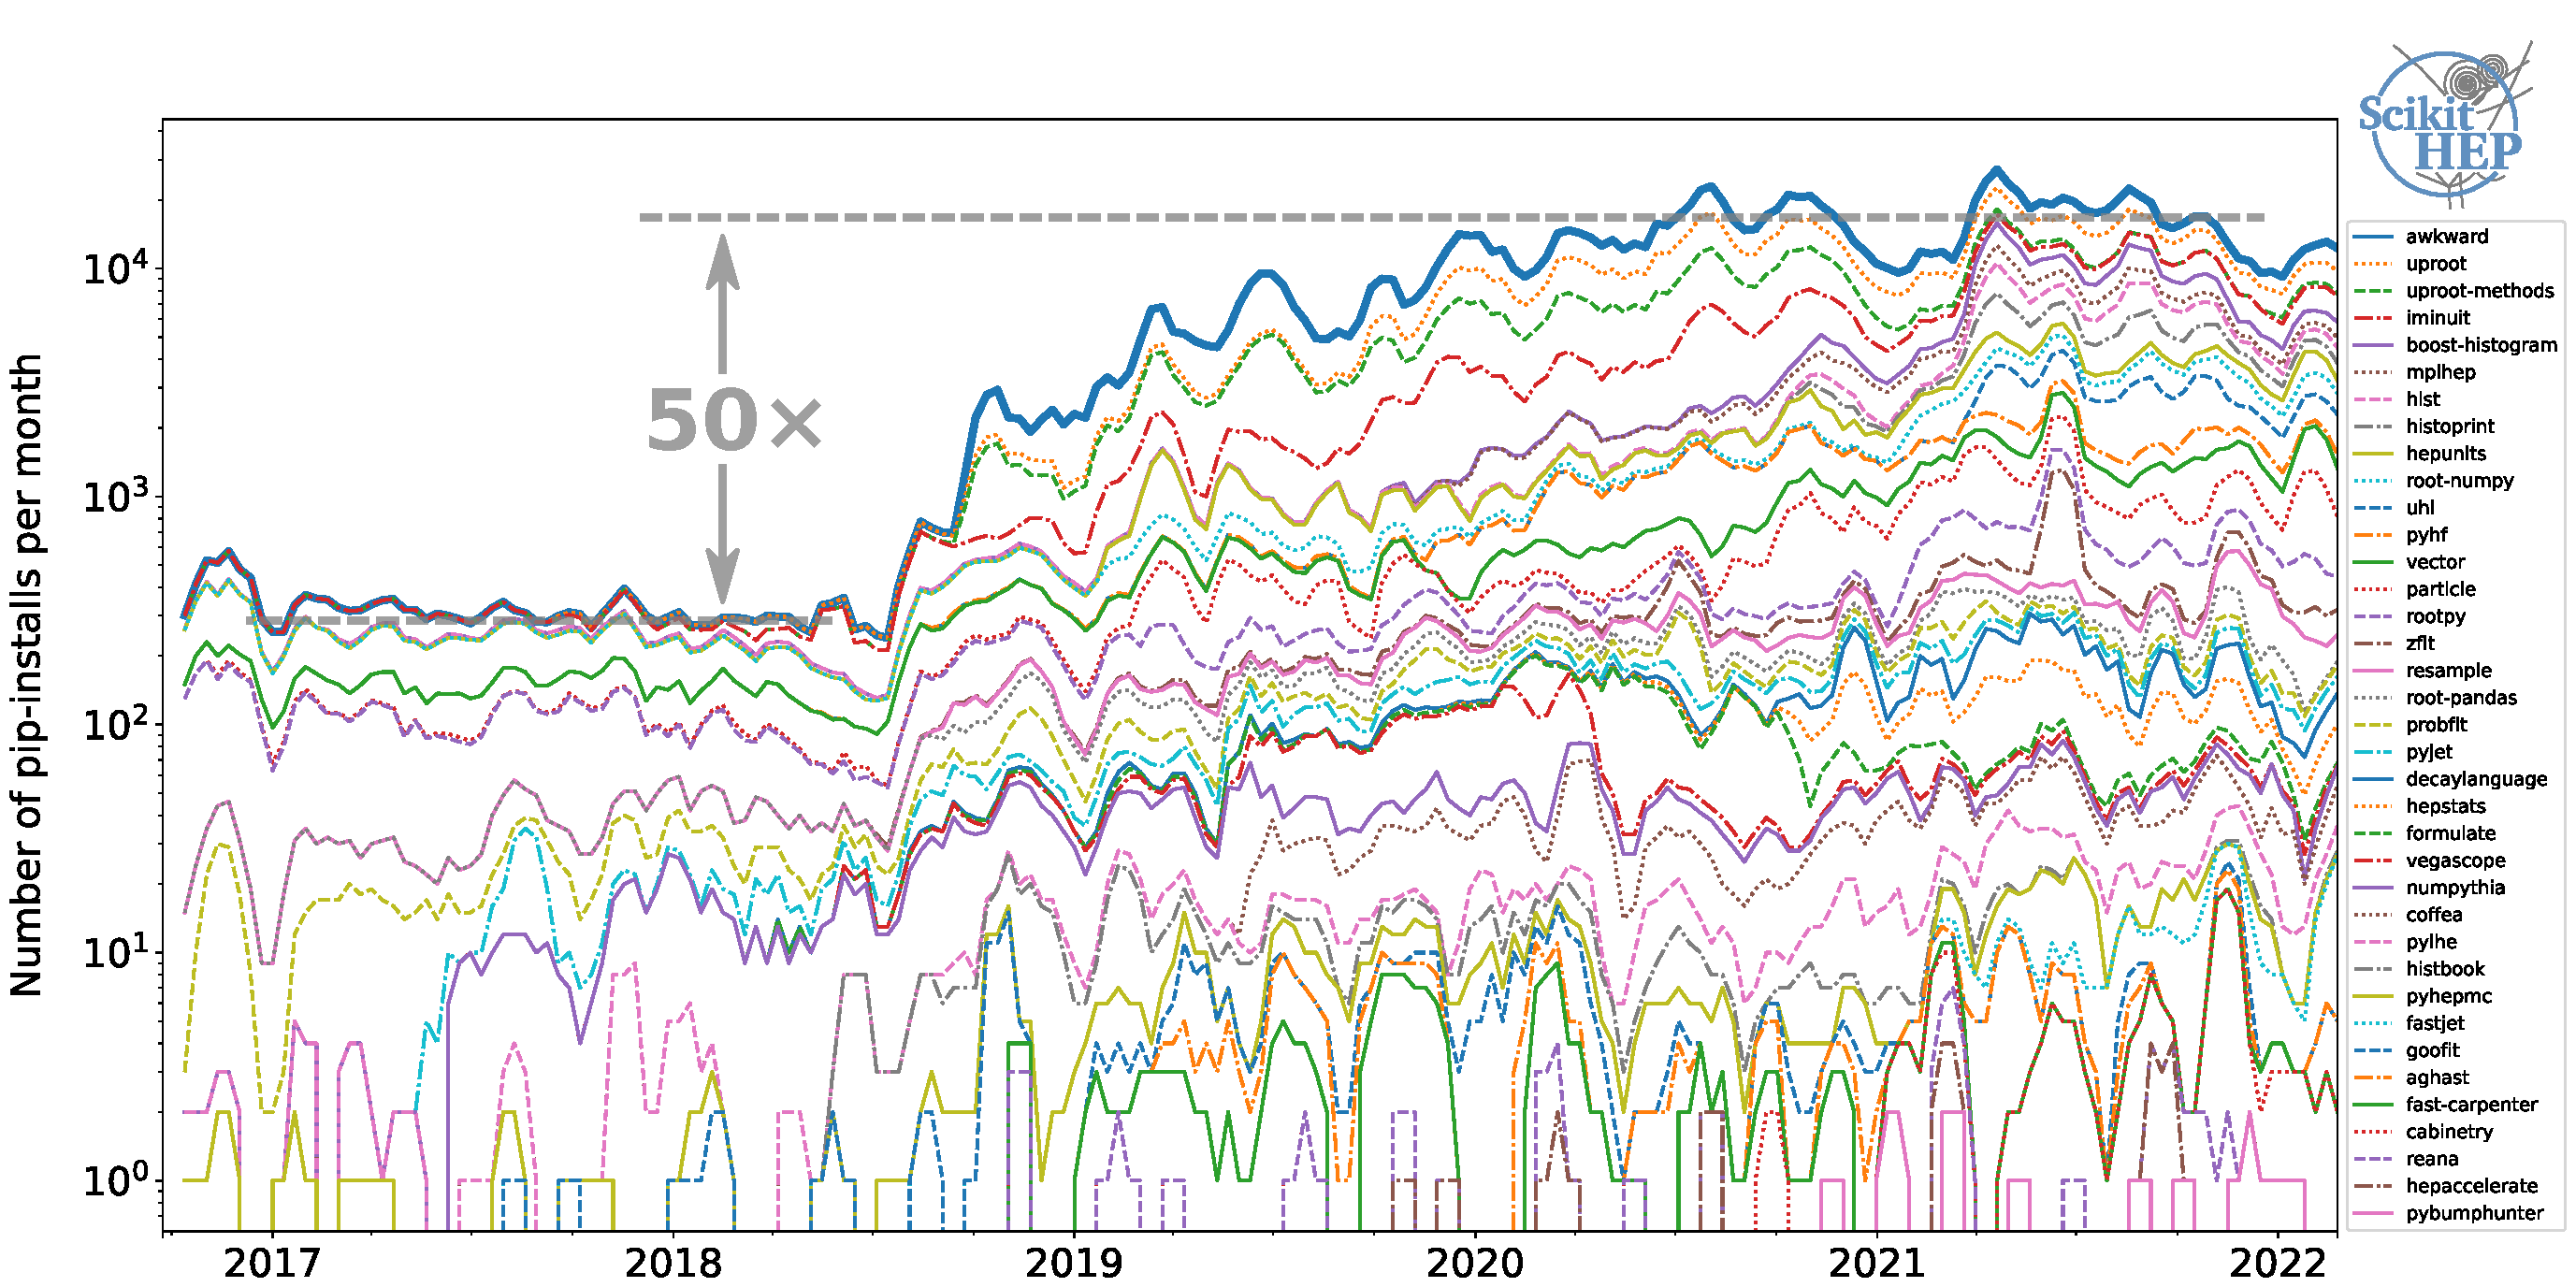
\includegraphics[width=\linewidth]{PLOTS/pip-macwin-scikithep-log-for-report.pdf}}
\end{frame}

\begin{frame}{}
\vspace{1 cm}
\Large

\begin{center}
There isn't a central authority to divide up the space of analysis problems and assign people to develop packages.

\vspace{1 cm}
But interested developers find underserved areas and build them up. Borders between them start vague and eventually get defined.
\end{center}
\end{frame}

\begin{frame}{Case study: development of histogram packages}
\large
\vspace{0.5 cm}

The scientific Python world lacked HEP-style histograms; it's one of the things we had to make ourselves.

\vspace{0.5 cm}
\uncover<2->{Also, it seems easy: just bin and count, right?}

\vspace{0.5 cm}
\uncover<3->{Physicists have created at least 20 histogram packages in Python, mostly by single authors.}

\vspace{0.5 cm}
\begin{uncoverenv}<3->
\begin{columns}
\scriptsize
\column{0.26\linewidth}
\begin{itemize}
\item PyROOT (2004--now)
\item PAIDA (2004--2007)
\item Plothon (2007--2008)
\item SVGFig (2008--2009)
\item YODA (2008--now)
\end{itemize}

\column{0.27\linewidth}
\begin{itemize}
\item DANSE (2009--2011)
\item rootpy (2011--2019)
\item SimpleHist (2011--2015)
\item pyhistogram (2015)
\item multihist (2015--now)
\end{itemize}

\column{0.28\linewidth}
\begin{itemize}
\item matplotlib-hep (2016)
\item QHist (2017--2019)
\item Physt (2016--now)
\item \mbox{Histogrammar (2016--now)\hspace{-0.2 cm}}
\item HistBook (2018--2019)
\end{itemize}

\column{0.32\linewidth}
\begin{itemize}
\item Coffea.hist (2019--2022)
\item boost-histogram (2019--now)
\item mplhep (2019--now)
\item histoprint (2020--now)
\item hist (2020--now)
\end{itemize}

\end{columns}
\end{uncoverenv}
\end{frame}

\begin{frame}{Histogram proliferation and convergence}
\large
\vspace{0.25 cm}

Number of unique developers contributing to each package per month (in git). Measures concentration of {\it developer activity}, not users.

\vspace{0.1 cm}
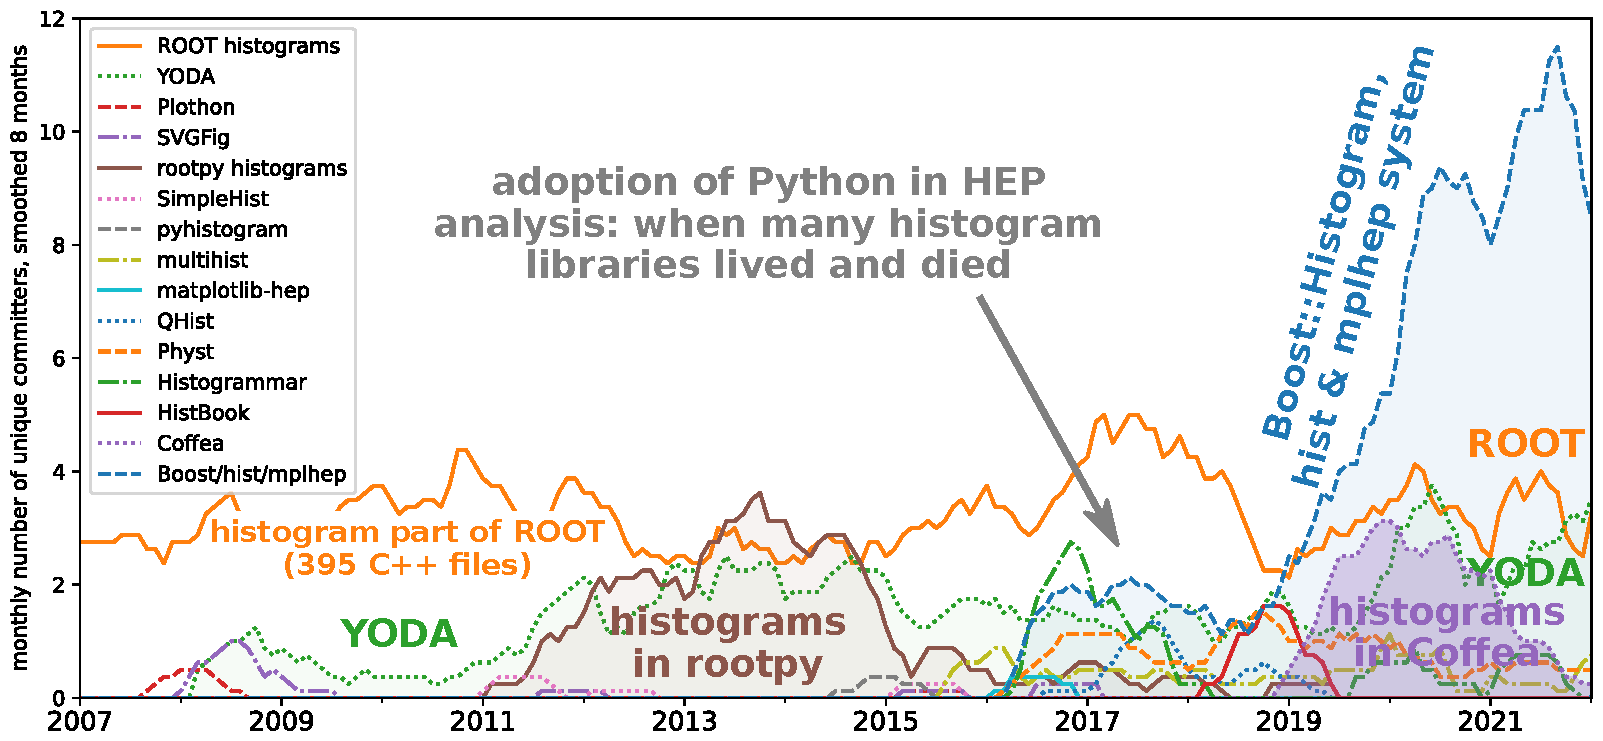
\includegraphics[width=\linewidth]{PLOTS/github-histogram-libraries.pdf}
\end{frame}

\begin{frame}[fragile]{Boost::Histogram, hist \& mplhep ``system''}
\vspace{0.5 cm}
\begin{columns}
\column{0.6\linewidth}
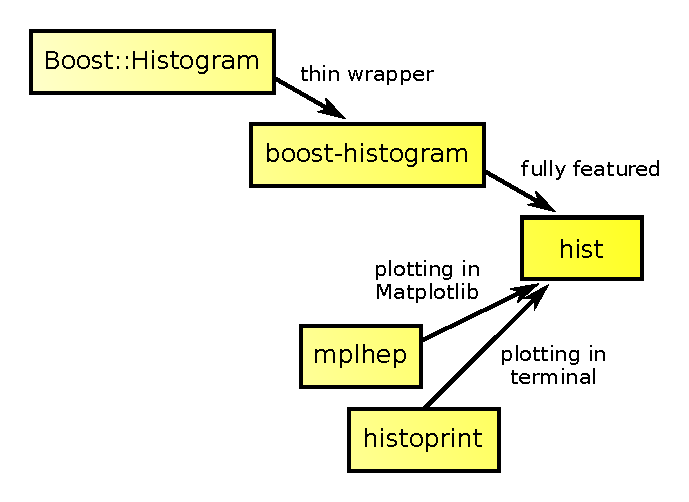
\includegraphics[width=\linewidth]{PLOTS/histogram-convergence.pdf}

\column{0.45\linewidth}
Originally, each of these was developed independently by a single author.

\vspace{0.75 cm}
\begin{uncoverenv}<2->
They each provide a piece of functionality users can get through

\begin{minted}{python}
import hist
\end{minted}
\end{uncoverenv}

\vspace{0.75 cm}
\uncover<3->{Now, 47 developers have contributed to these packages, and 20 contributed to more than one.}
\end{columns}
\end{frame}

\begin{frame}{Now we define the borders: agreed-upon protocols}
\vspace{0.5 cm}
\begin{columns}
\column{1.1\linewidth}
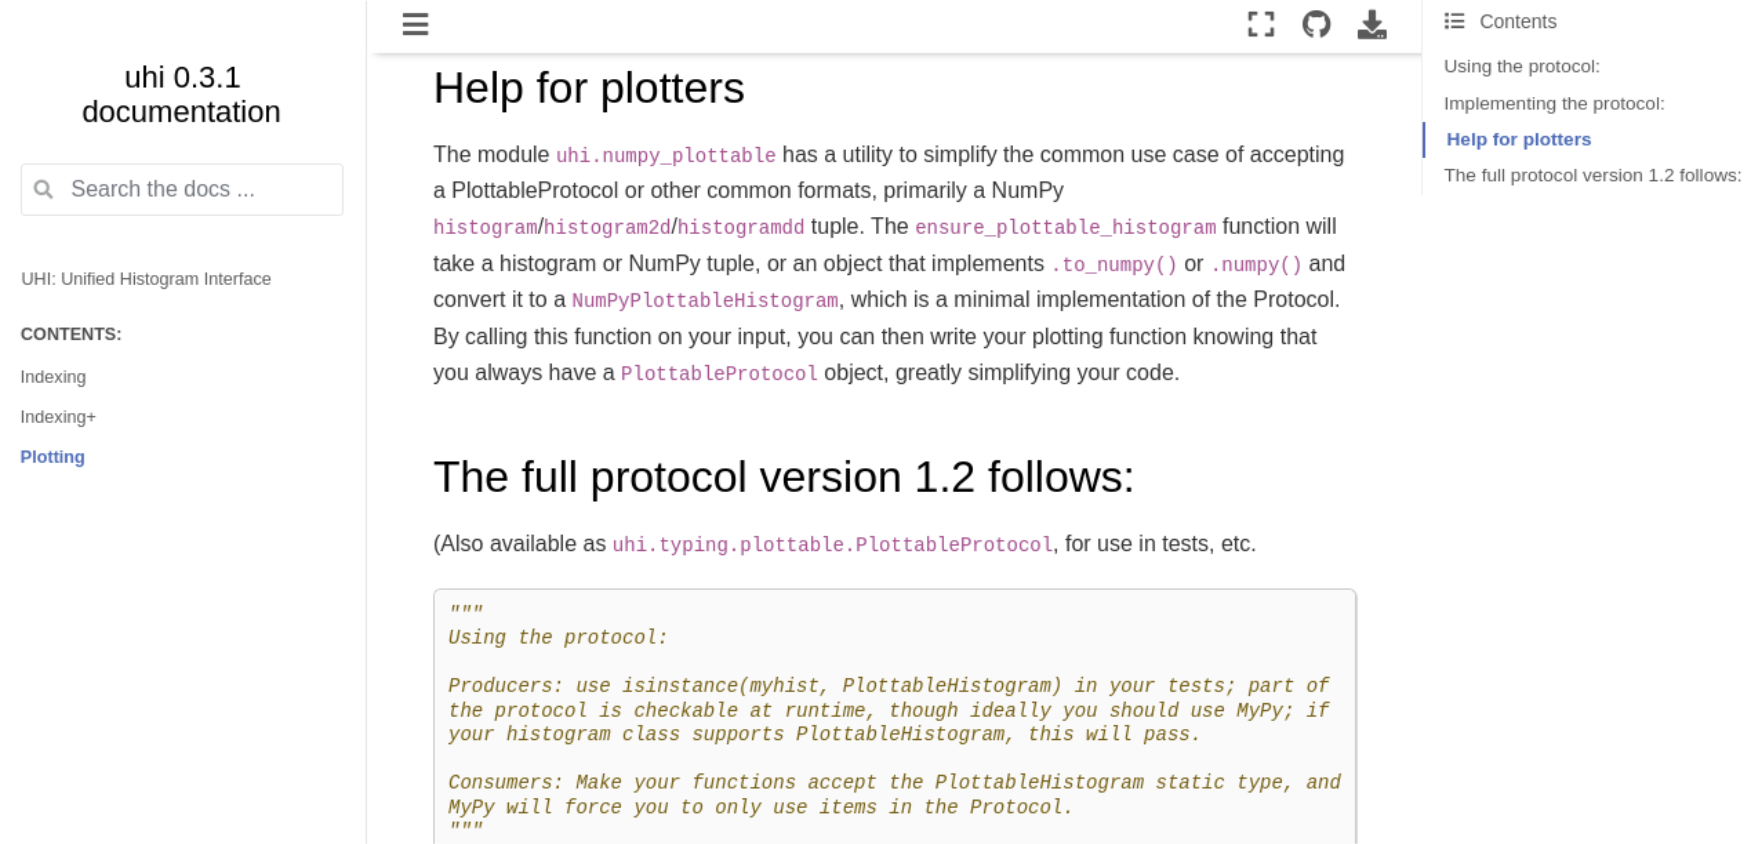
\includegraphics[width=\linewidth]{PLOTS/histogram-protocol-screenshot.png}
\end{columns}
\end{frame}

\begin{frame}{}
\vspace{1 cm}
\Large

\begin{center}
For users, the multiplicity of packages isn't a problem because package managers resolve dependencies.

\vspace{1 cm}
\texttt{\textbf{\textcolor{darkgreen}{pip install} \textcolor{blue}{hist}}}

\vspace{1 cm}
For developers, it provides more visibility, \\ ease of maintenance, and protection against scope-creep.
\end{center}
\end{frame}




\end{document}
